
\begin{figure}[t]
    \centering

    \subfloat[
        RISC-V assembly that demonstrates out-of-order execution.
    ]{
        \begin{minipage}{0.9\textwidth}
            \large
            \inputminted{gas}{media/code/OoO.S}
        \end{minipage}
        \vspace{4pt}
    }
    \vspace{4pt}

    \subfloat[
        Screenshot of WaveForm.
        \emph{(Note: this figure omits redundant cycles to improve readability)}.
    ]{
        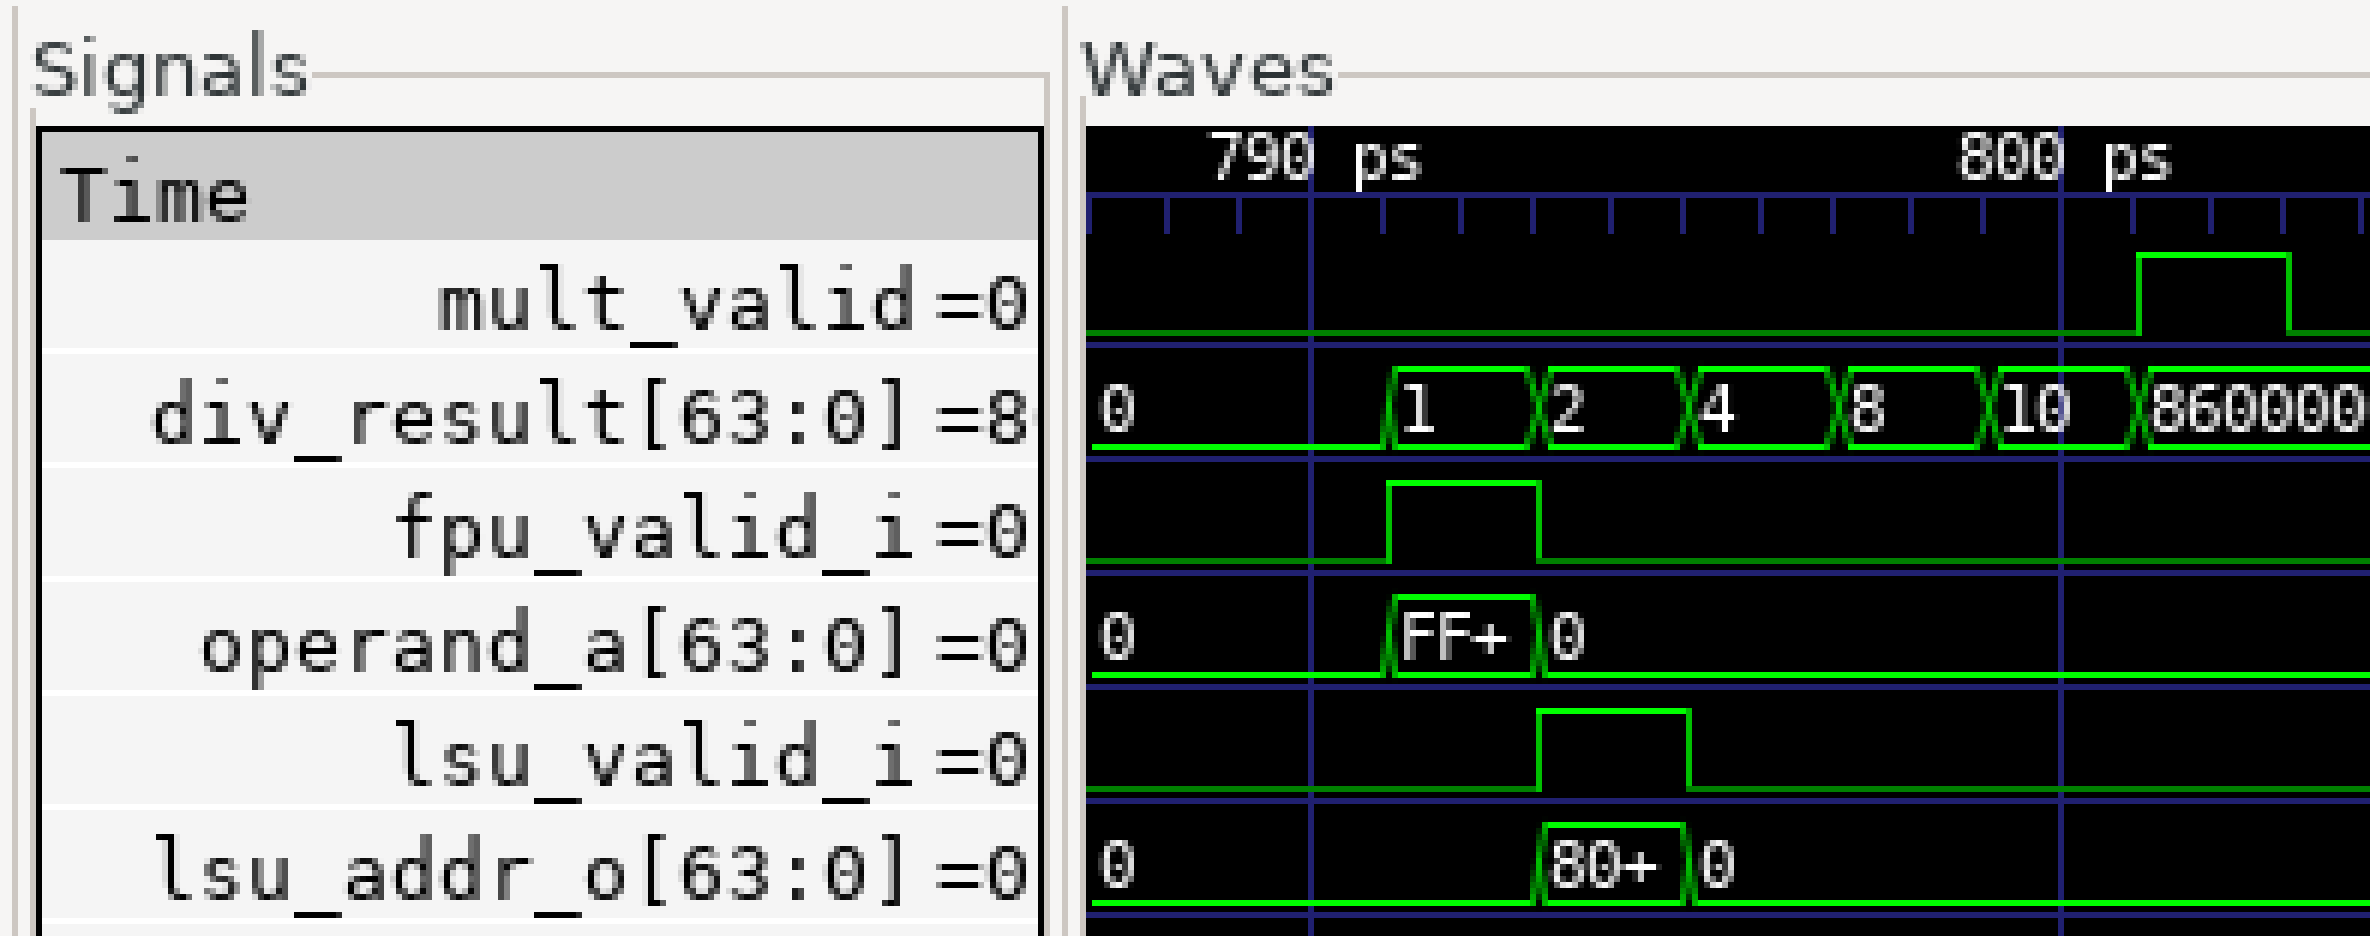
\includegraphics[width=0.9\linewidth]{media/graphics/labs_with_cva6/OoO.png}
    }
    \vspace{6pt}

    \caption[
        Out-of-Order Demonstration with CVA6
    ]{
        Out-of-Order Demonstration with CVA6: FPU and LSU finish before MULT \cite{SiffermanLatchUp}.
        In the Out-of-Order lab, participants are asked to write an assembly program to demonstrate code with and without different data-hazards.
    }
    \label{fig:OoO}

\end{figure}
